\part{Referencial Teórico}

\chapter[Extreme Programming]{Extreme Programming}

\section{Metodologias ágeis}

As abordagem de desenvolvimento de software vem mudando drasticamente na última década. Existem várias desvantagens acerca das metodologias tradicionais e bem documentadas, consideradas muito “pesadas” para algumas abordagens. Em resposta a essas abordagens, um novo grupo de metodologias têm aparecido nos últimos anos. Estas metodologias são as conhecidas como metodologias ágeis. \cite{Agarwal:2008}

As metodologias ágeis envolvem menos documentação e são mais focadas no código fonte do produto. Elas são mais adaptativas do que as consideradas “tradicionais”. Muitas metodologias hoje caminham para o lado ágil. Todas possuem características similares, mas também diferenças significativas. Entre as várias metodologias ágeis dos dias de hoje, podemos destacar o XP (Extreme Programming), Scrum e o Crystal.

Neste trabalho apenas nos aprofundaremos na metodologia XP. Seus fundamentos e princípios serão a base para a construção da metodologia e da definição do processo de desenvolvimento de software descritos no próximo capítulo deste trabalho.

\section{O que é o XP}

Segundo Kent Beck,  Extreme Programming (XP) é sobre mudança social. é sobre deixar ir embora nossos velhos hábitos e manias que antes faziam parte de uma adaptação forçada, mas que hoje em dia deixam de ser adaptação, para ser aquilo que define como fazer o nosso trabalho da melhor forma possível. é sobre abrir mão das defesas que nos protegem, mas interferem em nossa produtividade.

Extreme Programming (XP) é um estilo de desenvolvimento de software focado na excelência na aplicação de técnicas de programação, comunicação clara e trabalho em equipe. O XP também pode ser descrito como uma filosofia de desenvolvimento de software baseada em valores, sendo eles: comunicação, feedback, simplicidade, coragem e respeito.

Além dos valores, a filosofia de desenvolvimento do XP também possui princípios e suas práticas. O Extreme Programming nada mais é do que uma junção harmoniosa destas três vertentes. Kent Beck descreve em seu livro uma ponte, que representa os três elos presentes no XP. A figura abaixo representa a ponte descrita por Kent:

\begin{figure}[h]
	\centering
	\label{fig02}
		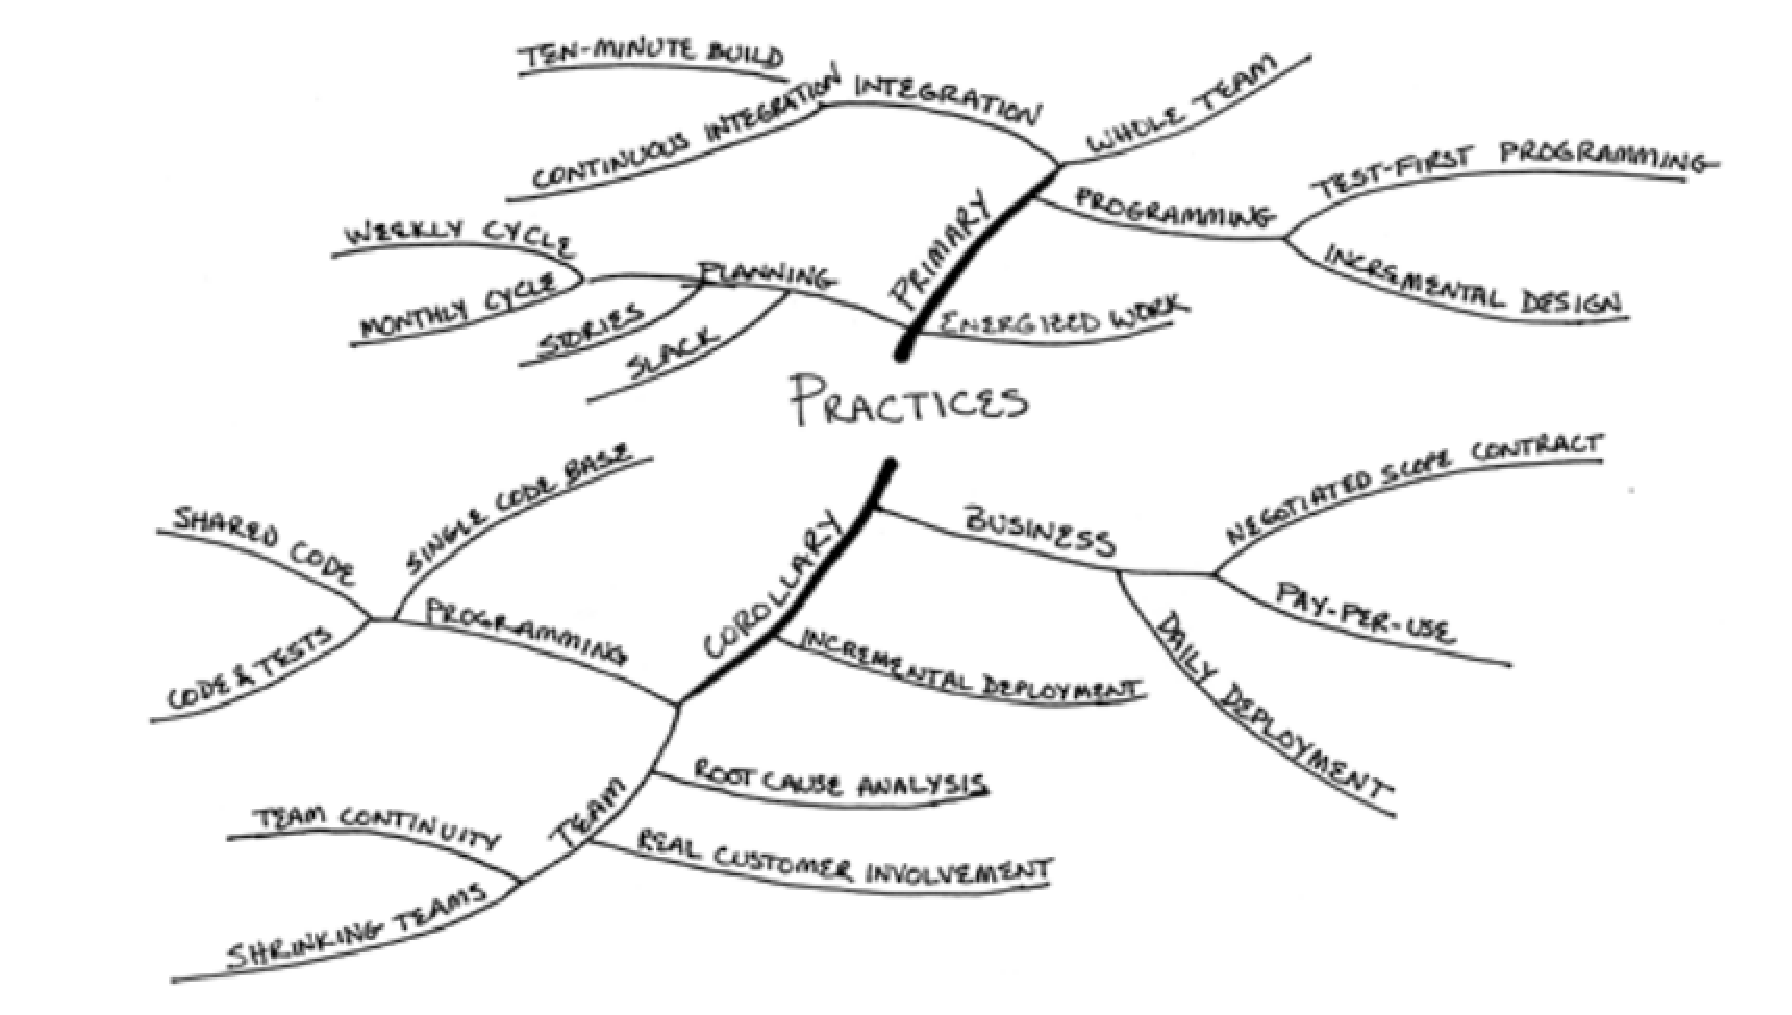
\includegraphics[keepaspectratio=true,scale=0.6]{figuras/fig02.eps}
	\caption{Representação Visual do XP. Fonte: Kent Beck, Extremme Programming Explained}
\end{figure}

A seguir serão descritas as características gerais do valores, os princípios do Extreme Programming, e uma explicação sobre todas as práticas propostas pela metodologia.

\section{Valores}

A comunicação é o fator mais importante em um time de desenvolvimento. Muitas vezes, quando um problema surge no desenvolvimento, certamente algum membro do time já tem a resposta para o mesmo. A falta da comunicação é aquilo que impede a transformação desta solução em código por alguém que teria a capacidade técnica para tal implementação.

Simplicidade pode ser considerada o valor mais “inteligente” dentro do XP. Fazer um sistema simples, de fácil entendimento e manutenção é uma tarefa árdua. Focar em resolver os problemas de “hoje” de uma forma graciosa o suficiente para que o amanhã não seja um problema é o objetivo principal da metodologia. Em poucas palavras: Devemos saber facilmente onde estamos e uma maneira simples de chegar onde queremos.

Definir as direções de um projeto antes de adquirir a experiência necessária para tal tarefa pode gerar mudanças. Quando falamos de mudança dentro do desenvolvimento de software podemos estar falando dos requisitos, da arquitetura do sistema ou mesmo do código fonte. Mudanças dentro do projeto fazem surgir a necessidade de feedback.

O feedback pode ser um mecanismo efetivo para a equipe se aproximar de suas metas. Ele pode se manifestar de várias formas, algumas delas são:

\begin{itemize}

\item Opiniões sobre uma ideia, debatendo com seu time sobre a viabilidade da mesma;

\item Como implementar uma ideia no código e como seria o estado do mesmo após essa implementação;

\item As dificuldades para o deploy deste código após a resolução de um problema;

\item A melhor forma de testar um trecho de código fonte;

\end{itemize}

Os times devem ser capazes de absorver a maior quantidade de feedback possível. Quanto mais cedo um problema é descoberto, mais rápido ele será solucionado.

A solução rápida dos problemas nos remete a outro valor presente no XP, a coragem. Quando os desenvolvedores se deparam com problemas, tomar uma atitude e resolvê-lo o mais rápido possível é encorajado pela metodologia. Entretanto, essa atitude não deve ser tomada sem o conhecimento do time ou sem pensar no benefício do mesmo. Uma coragem “individualista” não leva a bons resultados dentro do projeto.

Os valores tem a intenção de balancear e ser o suporte entre eles próprios. Melhorar a sua comunicação com a equipe pode ajudar a alcançar a simplicidade desejada dentro do seu projeto. Alcançar essa simplicidade dá ao desenvolvedor menos motivos para que as conversas entre o time se estendam por mais tempo do que deveriam.

Por fim, Kent Beck reforça a importância do respeito dentro do desenvolvimento de software. Para ele, é o valor que suporta todos os outros 4. Se os outros membros do time não ligam para sua equipe e não respeitam a opinião da mesma, o projeto nunca poderá ser bem sucedido.

\section{Princípios}

O Extreme Programming também preza por príncipios. Estes podem ser considerados tão abstratos quanto os valores citados na seção anterior. Como a explicação sobre cada um deles é extensa e sua interpretação pode ser mais complexa para alguns, nesta parte apenas serão citados com uma breve descrição baseada na metodologia e na análise de Kent em seu livro:

\begin{enumerate}

	\item Humanidade: O XP e as metodologias ágeis como um todo tem seu foco no aspecto humano. As necessidades das pessoas e são colocadas ao lado das necessidades do time. Afinal, software é desenvolvido por pessoas.

	\item Aspecto Econômico: é fundamental entender que todo o desenvolvimento deve ser feito pensando no aspecto de “valor”. Valor para o negócio, para o cliente, para o time e para a sociedade como um todo. Pensar em soluções que sejam válidas em um futuro próximo também é pensar em aspectos econômicos.

	\item Benefício Mútuo:  O princípio mais complexo de ser cumprido dentro dos times. Sempre que tomamos uma decisão técnica, estamos pensando no benefício de um fator em detrimento de outro. Um bom exemplo  de como a aplicação deste princípio é complexa seria a construção de um código já pensando na manutenção do mesmo por outra pessoa. A tarefa de pensar em soluções que sempre beneficiam todas as partes envolvidas pode ser exaustiva em vários casos.

	\item Melhoria:  Não existem processos perfeitos, códigos perfeitos ou o design perfeito. Tudo pode e deve ser melhorado. Refatoração de código e melhorias arquiteturais ou de design são fundamentais e encorajadas pela metodologia.

	\item Reflexão:   Bons time e bons desenvolvedores sempre devem refletir sobre o trabalho que estão executando, analisar falhas e acertos. Práticas do XP como pareamento e integração contínua são fundamentais na prática de reflexão dentro do ambiente de trabalho.

	\item Oportunidades: Enxergar os problemas durante o desenvolvimento de software como oportunidades de mudança. Nestes momento o desenvolvedor pode entender o que melhorar e como mudanças podem ser benéficas ao time.

 	\item Qualidade: O foco na qualidade é necessário para uma maior taxa de entrega de produto. Ao contrário do que se pode pensar, um produto com baixa qualidade pode ter seu desenvolvimento mais rápido no início, entretanto a taxa de entrega tem a tendência a decair no futuro conforme os problemas gerados pela baixa qualidade do produto vão emergindo.

	\item Baby-Steps: Em uma metodologia que busca abraçar mudanças, muitas delas podem ser grandes e impactantes. O desgaste do time desenvolvendo solução em pequenos passos é sempre menor do que a perda de tempo do mesmo corrigindo erros ou abortando grandes passos.

\end{enumerate}



\chapter[Tamanho Funcional de Software]{Tamanho Funcional de Software}

Este capítulo descreve o surgimento da contagem de tamanho funcional, a técnica de contagem de pontos de função (IFPUG) pelo manul do CPM.

\section{Tamanho Funcional de Software}

A contagem de tamanho funcional de software surgiu no ano de 1979, com Albrecht. A proposta era estimar o tamanho de um software a partir das funcionalidades entregues ao usuário. Estas primeiras métricas ficaram conhecidas como Function Points(FP)  e  Function Points Analysis (FPA)  e eram uma alternativa para suprir o problema da indústria em estimar prazos e esforço necessário para a o desenvolvimento de software.

Nos anos seguintes surgiram várias propostas de melhoria e variações do modelo apresentado no ano de 1979. No ano de 1986 a International Function Point User Group (IFPUG) foi criada como uma organização sem fins lucrativos. Sua função era, entre algumas outras, a de promover e disseminar o gerenciamento de projetos através do uso de FPA. Em 1996 a International Organization for Standardization (ISO), estabeleceu princípios de comum entendimento e uma interpretação consistente das  definições que permeiam a medição de tamanho funcional. Atualmente a ISO/IEC 20926:2010 regulamenta a análise de pontos de função. Ela define regras e etapas para aplicação da mesma em projetos de desenvolvimento e manutenção de software.

\section{Contagem de Pontos de Função}

O manual de contagem do IFPUG descreve o procedimento de contagem de pontos de função a partir de alguns passos:

\begin{itemize}

\item Definir as fronteiras de medição, o escopo e o propósito da mesma. A fronteira de um software pode ser definida estabelecendo uma fronteira lógica entre o software a ser medido, seus usuários e a interação com outros softwares. Essa fronteira pode ser subjetiva, consequentemente tornando difícil a delimitação do início de um software e do término de outro.

\item Medir as funções de dados. Uma função de dados refere-se aos requisitos na visão do usuário em relação ao armazenamento e a referência de dados da aplicação. Podem ser classificadas em arquivos lógicos interno e externos.

\item Medir as funções de transação. Estas funções são caracterizadas pelo processamento de dados por uma funcionalidade provida ao usuário. Podemos classificá-las em três tipos: saída externa, entrada externa e consulta externa e definir a complexidade de cada uma como baixa, média e alta.

\item Calcular o tamanho funcional. A partir da soma da complexidade das funções da dos e das funções de transação é possível calcular um tamanho total em pontos de função de um software. Vale ressaltar que existem aspectos para ajustar os pontos de função de acordo com a necessidade do projeto.

\item Reportar os resultados. O último passo listado pelo manual corresponde ao relato dos resultados obtidos pela contagem, além de interpretações e possíveis tomadas de decisões a partir dos valores obtidos.

\end{itemize}

A figura a seguir representa os passos descritos anteriormente para a realização do procedimento de contagem de pontos de função:

\begin{figure}[h]
	\centering
	\label{fig01}
		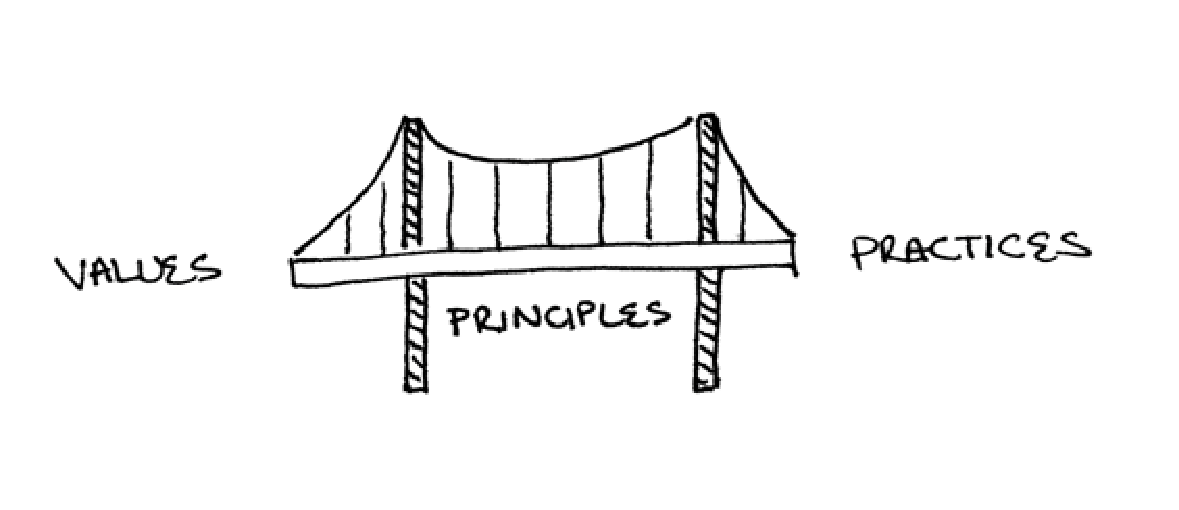
\includegraphics[keepaspectratio=true,scale=0.4]{figuras/fig01.eps}
	\caption{Processo de contagem de pontos de função. Fonte: Roteiro de métricas do SISP}
\end{figure}


As tabelas abaixo descrevem a pontuação de funções de dados e funções de transação de acordo com a complexidades medidas durante a contagem:





Apesar da eficiência da contagem de pontos de função, ao longo dos anos estudos foram feitos a fim de descobrir problemas, lacunas do processo e possíveis melhorias para o mesmo. Buscando saber quais seriam esses problemas e alternativas para solucionar essas lacunas, em 2015 três autores brasileiros realizaram um processo de revisão sistemática na literatura para agrupar as observações feitas por outros autores na área.

Os autores classificaram os problemas encontrados em três tipos: Peso e complexidade, independência de tecnologia e ajuste da pontuação. As principais críticas a parte de peso e complexidade da contagem de pontos de função diz respeito a mesma classificação em complexidade de duas funções de transação ou de dados com diferentes quantidades de campos e referências a arquivos. Outra crítica seria o espaçamento entre as complexidades. Alguns autores acreditam que definir apenas como baixa, média e alta pode ser muito e alto e acabar não detalhando de forma mais aproximada a real complexidade de desenvolvimento de uma funcionalidade.

Problemas relacionados a independência de tecnologia também são citados na revisão sistemática feita pelos autores. O principal questionamento dos pesquisadores é a falta de adaptação do processo de contagem às novas linguagens de programação. A abordagem não reflete o atual desenvolvimento de software, principalmente o advento e crescimento da orientação a objetos. A independência de tecnologias também diz respeito ao hardware, muito diferente hoje do que a existente a 20 anos atrás.

Por fim, o estudo relata problemas como ajuste do ponto de função. Alguns autores afirmam que o ajuste não considera  importantes requisitos não funcionais, dentre eles: usabilidade, manutenibilidade, eficiência, e portabilidade.

Mesmo com os problemas e lacunas descobertos ao longo dos anos, a indústria de desenvolvimento de software continuam usando a contagem de pontos de função para a estimativa de tamanho de software.Na visão de Ebert \cite{Ebert:2014}, as companhias passaram a adotar esse modelo de estimativa com algumas finalidades. A primeira delas seria alocar melhor os recursos a partir de uma primeira estimativa de prazo e esforço necessário para a produção. Outro fator seria a estimativa de esforço quando alguma mudança nos requisitos do projeto ocorresse. Além disso também seria possível medir a produtividade e taxas de entrega de software, possibilitando benchmarks  e análises de pontos de melhoria no processo de desenvolvimento.

A utilização dos pontos de função para estimativas de projeto passou a ser usada também por órgãos de governo e não só por companhias ou fábricas de desenvolvimento de software. O Roteiro de Métricas de Software(2016) do SISP cita essa utilização do processo em órgãos e em empresas privadas, além dos benefícios obtidos por ambos pela utilização dos mesmo:  “Diversas instituições públicas e privadas têm utilizado a métrica Ponto de Função(PF) nas estimativas e dimensionamento de tamanho funcional de projetos de software devido aos diversos benefícios de utilização desta métrica, destacando-se: regras de contagem objetivas, independência da solução tecnológica utilizada e facilidade de estimativa nas fases iniciais do ciclo de vida do software.”
